\chapter{Metabolisme Mikroba dan Biofilm}\label{ch:b2:microbial-metabolism}

Isilah sebuah tabung kaca dengan lumpur kolam, sedikit kertas cacahan,
sebutir kuning telur, dan air, lalu letakkan di ambang jendela. Dalam
beberapa pekan tabungnya berlapis menjadi pita berwarna: alga hijau di
puncaknya, sebuah lapisan berkarat, sebuah pita ungu, sebuah pita hijau
lebih ke bawah, dan lumpur sulfida hitam di dasarnya. Tidak ada yang
ditambahkan kecuali cahaya. Tiap pitanya adalah satu populasi yang
hidup dari kimia yang berbeda --- dari oksigen, nitrat, sulfat,
sulfida, hidrogen --- dan masing-masing menyuapi pita berikutnya.
Tabung itu adalah dunia mikroba dalam ukuran kecil: sel yang meraih
energinya dari hampir setiap pasangan zat yang dapat bertukar elektron,
dan yang, bersama-sama, menjalankan daur kimia planet ini. Bab ini
memaparkan tata nalar energetika itu, kinetika pertumbuhan mikroba, dan
kehidupan bersama mikroba pada permukaan, yang merupakan cara hidup
sebagian besar mereka.

\section{Cara-cara mencari nafkah}

\begin{definition}[Tipe trofik]\label{def:b2:microbial-metabolism:trophic}
\index{kemotrof}\index{fototrof}\index{litotrof}\index{organotrof}
Sebuah organisme digolongkan lewat tiga jawaban. \emph{Sumber
energi}nya: cahaya (\emph{fototrof}) atau reaksi kimia
(\emph{kemotrof}). \emph{Sumber elektron}nya: zat anorganik ---
$\mathrm{H_2}$, $\mathrm{H_2S}$, $\mathrm{NH_4^+}$,
$\mathrm{Fe^{2+}}$, air --- (\emph{litotrof}) atau molekul organik
(\emph{organotrof}). \emph{Sumber karbon}nya: $\mathrm{CO_2}$
(\emph{autotrof}) atau karbon organik (\emph{heterotrof}). Tumbuhan
dan sianobakteri adalah fotolitoautotrof; hewan, fungi, dan
\emph{E.~coli} adalah kemoorganoheterotrof; bakteri penitrifikasi dan
pengoksidasi belerang adalah kemolitoautotrof, yang membuat bahan
organiknya dari $\mathrm{CO_2}$ dengan energi yang ditarik dari
oksidasi mineral, di dalam gelap. Hampir setiap gabungannya ada di
suatu tempat di antara \omterm{def:b2:unicellular-diversity:prokaryote}{prokariot}; eukariot hanya menempati dua.
\end{definition}

\begin{theorem}[Energi sepasang redoks]\label{thm:b2:microbial-metabolism:redox}
\index{potensial redoks}\index{menara elektron}
Setiap metabolisme penghasil energi memindahkan elektron dari sepasang
\emph{pemberi} ke sepasang \emph{penerima}. Tiap pasangan memiliki
potensial baku $E^{\circ\prime}$ (pada pH 7): makin negatif, makin
mudah ia memberikan elektron. Memindahkan $n$ mol elektron dari pemberi
pada $E_d$ ke penerima pada $E_a$ melepaskan energi bebas baku
\[
\Delta G^{\circ\prime} = -\,n F\,(E_a - E_d), \qquad F = \qty{96.5}{kJ/V/mol},
\]
sehingga hasilnya sebanding dengan jarak tegak antara kedua pasangan
itu pada \emph{\omterm{thm:b2:microbial-metabolism:redox}{menara elektron}}. Dengan
$\mathrm{O_2/H_2O}$ pada \qty{+0.82}{V} dan $\mathrm{CO_2}$/glukosa pada
\qty{-0.43}{V}, ke-24 elektron sebuah molekul glukosa menghasilkan
$24\times 96.5\times 1.25 = \qty{2900}{kJ/mol}$; diserahkan kepada
sulfat ($\mathrm{SO_4^{2-}/H_2S}$, \qty{-0.22}{V}), elektron yang sama
hanya menghasilkan $24\times 96.5\times 0.21 = \qty{490}{kJ/mol}$.
\end{theorem}
\begin{proof}
Bagi reaksi pemberi$_{\text{tereduksi}}$ + penerima$_{\text{teroksidasi}}$
$\to$ pemberi$_{\text{teroksidasi}}$ + penerima$_{\text{tereduksi}}$, perubahan energi
bebasnya adalah kerja yang dilakukan oleh muatan $n$ mol elektron $nF$
yang jatuh menempuh selisih potensial $E_a - E_d$, dengan kesepakatan
tanda bahwa pemindahan spontan (elektron menuju pasangan yang lebih
positif) memiliki $\Delta G < 0$. Inilah hubungan Nernst dari jilid
Tahun ke-1 yang diterapkan pada dua setengah reaksi.
\end{proof}

\begin{omfigure}
\begin{tikzpicture}[every node/.style={font=\scriptsize}, y=6cm]
  \draw[thick, ->] (0,-0.55) -- (0,0.95) node[above] {$E^{\circ\prime}$ (V)};
  \foreach \v in {-0.4,-0.2,0,0.2,0.4,0.6,0.8} \draw (-0.08,\v) -- (0.08,\v) node[right, xshift=0.05cm] {\v};
  % donors on the right: value/label position/text
  \foreach \v/\y/\l in {-0.43/-0.49/{$\mathrm{CO_2}$/glukosa}, -0.42/-0.40/{$2\mathrm{H^+/H_2}$}, -0.32/-0.31/{$\mathrm{NAD^+/NADH}$}, -0.27/-0.22/{$\mathrm{S^0/H_2S}$}, 0.03/0.03/{fumarat/suksinat}, 0.34/0.34/{$\mathrm{NO_2^-/NH_4^+}$}}
    { \draw[omDef, thick] (0.8,\v) -- (1.6,\v); \draw[omDef] (1.6,\v) -- (1.85,\y); \node[omDef, anchor=west] at (1.9,\y) {\l}; }
  % acceptors on the left
  \foreach \v/\y/\l in {-0.24/-0.29/{$\mathrm{CO_2/CH_4}$}, -0.22/-0.17/{$\mathrm{SO_4^{2-}/H_2S}$}, 0.43/0.43/{$\mathrm{NO_3^-/NO_2^-}$}, 0.74/0.69/{$\mathrm{NO_3^-/N_2}$}, 0.77/0.77/{$\mathrm{Fe^{3+}/Fe^{2+}}$}, 0.82/0.86/{$\mathrm{O_2/H_2O}$}}
    { \draw[omThm, thick] (-1.6,\v) -- (-0.8,\v); \draw[omThm] (-1.6,\v) -- (-1.85,\y); \node[omThm, anchor=east] at (-1.9,\y) {\l}; }
  \node[omThm, anchor=south] at (-2.4,0.93) {penerima};
  \node[omDef, anchor=south] at (2.4,0.93) {pemberi};
  % arrows showing two metabolisms
  \draw[->, very thick, omExo!80!black] (4.9,-0.43) -- (4.9,0.80);
  \node[anchor=west, align=left] at (5.0,0.2) {respirasi aerob\\glukosa: \qty{1.25}{V},\\\qty{2900}{kJ/mol}};
  \draw[->, very thick, omProp] (4.2,-0.43) -- (4.2,-0.24);
  \node[anchor=north, align=center] at (4.2,-0.52) {reduksi sulfat:\\\qty{0.21}{V}, \qty{490}{kJ/mol}};
  \draw[dashed, gray] (3.5,-0.43) -- (4.9,-0.43);
  \draw[dashed, gray] (3.5,0.82) -- (4.9,0.82);
  \draw[dashed, gray] (3.5,-0.22) -- (4.2,-0.22);
\end{tikzpicture}

{\small \omterm{thm:b2:microbial-metabolism:redox}{Menara elektron}. Pemberi (biru) didaftar pada potensial
bakunya; penerima (merah) demikian pula. Sebuah metabolisme adalah
jatuhan dari seorang pemberi ke seorang penerima di atasnya, dan hasil
energinya sebanding dengan tinggi jatuhannya: glukosa ke oksigen adalah
jatuhan yang panjang, glukosa ke sulfat jatuhan yang pendek.}
\end{omfigure}

\begin{proposition}[Kemolitotrofi]\label{prop:b2:microbial-metabolism:lithotrophy}
\index{kemolitotrofi}\index{nitrifikasi}
Sebagian bakteri menarik seluruh energinya dari oksidasi anorganik,
memakai oksigen (atau nitrat) sebagai penerima, dan memfiksasi
$\mathrm{CO_2}$ dengan ATP dan daya pereduksi yang diperolehnya.
\emph{Penitrifikasi}: pengoksidasi amonium
(\emph{Nitrosomonas}) mengubah $\mathrm{NH_4^+}$ menjadi nitrit
($\Delta G^{\circ\prime} = \qty{-275}{kJ/mol}$), pengoksidasi nitrit
(\emph{Nitrobacter}) mengubah nitrit menjadi nitrat (\qty{-74}{kJ/mol});
bersama-sama mereka mengubah amonium hasil pembusukan menjadi nitrat
yang diserap tumbuhan (\cref{ch:b2:biogeochemical-cycles}).
\emph{Pengoksidasi belerang} (\emph{Thiobacillus}, \emph{Beggiatoa})
mengoksidasi $\mathrm{H_2S}$ menjadi belerang dan sulfat;
\emph{pengoksidasi besi} mengoksidasi $\mathrm{Fe^{2+}}$ menjadi karat;
\emph{pengoksidasi hidrogen} membakar $\mathrm{H_2}$. Karena pemberi
elektronnya duduk tinggi pada menaranya, hasil tiap molekulnya kecil,
dan karena pemberinya adalah pereduksi yang lebih lemah daripada NADH,
mereka harus membelanjakan energi untuk mendorong elektron \emph{ke
atas} demi membuat NADH yang dibutuhkan fiksasi karbon: seorang
penitrifikasi mengoksidasi sekitar tiga puluh ion amonium untuk
memfiksasi satu $\mathrm{CO_2}$, dan tumbuh lambat.
\end{proposition}
\begin{proof}[Bukti eksperimental]
Winogradsky (1887--1890) menumbuhkan bakteri belerang berfilamen di
dalam setetes air yang ia biarkan dimasuki sulfida secara difusi dari
satu sisi dan udara dari sisi lainnya: mereka berkumpul di batasnya,
menimbun butiran belerang, lalu memakannya ketika sulfidanya diputus.
Ia kemudian mengisolasi bakteri penitrifikasi pada medium mineral murni
berisi amonium dan sama sekali tanpa karbon organik, dan di situ mereka
tumbuh serta menghasilkan nitrat --- peragaan pertama bahwa kehidupan
dapat dibangun dari $\mathrm{CO_2}$ dan energi sebuah reaksi anorganik,
tanpa cahaya. Ia menyebutnya kemosintesis.
\end{proof}

\begin{omfigure}
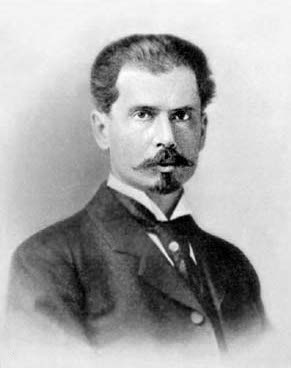
\includegraphics[width=0.26\linewidth]{images/book4/winogradsky.jpg}\hspace{0.05\linewidth}
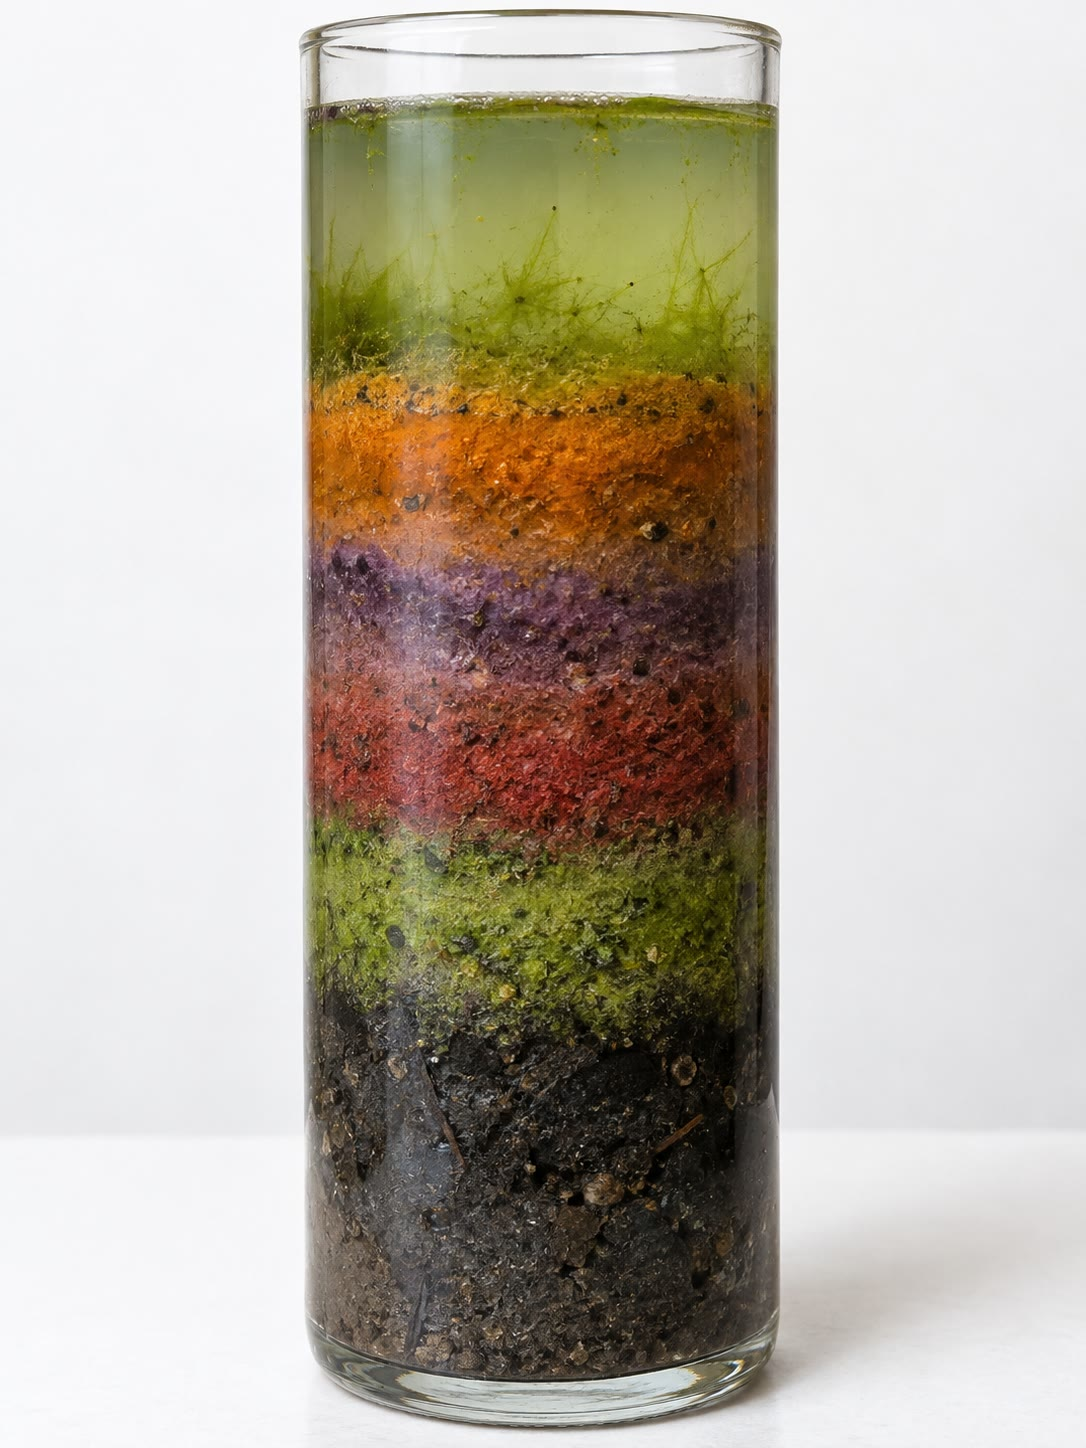
\includegraphics[width=0.30\linewidth]{images/book4/ai/b4-02-winogradsky-column.jpg}

{\small Sergei Winogradsky, penemu \omterm{def:b2:microbial-metabolism:trophic}{kemolitotrofi}, dan tabung
yang menyandang namanya: sebuah silinder lumpur dan air yang berlapis
di bawah cahaya menjadi pita alga, pengoksidasi besi dan belerang,
bakteri belerang ungu dan hijau, serta pereduksi sulfat di lumpur hitamnya.}
\end{omfigure}

\begin{definition}[Fotosintesis anoksigenik]\label{def:b2:microbial-metabolism:anoxygenic}
\index{fotosintesis anoksigenik}
Bakteri ungu dan hijau berfotosintesis dengan satu fotosistem tunggal
dan sebuah bakterioklorofil yang menyerap di inframerah dekat, memakai
$\mathrm{H_2S}$, $\mathrm{H_2}$, atau asam organik sebagai pemberi
elektron dan bukan air: mereka melepaskan belerang atau sulfat, tidak
pernah oksigen, dan mereka membutuhkan cahaya berpanjang gelombang yang
lolos melalui lapisan hijau dan sianobakteri di atasnya. Maka bakteri
belerang ungu tumbuh di pita ungu tabung Winogradsky, tepat di tempat
sulfida dari bawah bertemu cahaya dari atas; bakteri belerang hijau,
yang lebih tahan sulfida dan lebih hemat cahaya, tumbuh di bawahnya.
Fotosintesis beroksigen, dengan dua fotosistemnya yang tersusun seri,
adalah penemuan kemudian oleh satu garis keturunan --- sianobakteri ---
yang belajar mengambil elektron dari air.
\end{definition}

\section{Respirasi anaerob dan fermentasi}

\begin{definition}[Respirasi anaerob]\label{def:b2:microbial-metabolism:anaerobic}
\index{respirasi anaerob}\index{denitrifikasi}\index{reduksi sulfat}\index{metanogenesis}
\emph{Respirasi anaerob} adalah respirasi --- sebuah rantai
pengangkutan elektron yang memompa proton dan membuat ATP secara
kemiosmosis --- dengan penerima akhir selain oksigen.
\emph{Penitrifikasi balik} (\emph{Pseudomonas}, \emph{Paracoccus})
mereduksi nitrat menjadi nitrit, nitrogen monoksida, dinitrogen
monoksida, dan akhirnya $\mathrm{N_2}$, yang lolos ke udara; mereka
memakai rantai aerobnya dengan beberapa enzim tambahan dan beralih ke
nitrat hanya ketika oksigennya habis. \emph{Pereduksi sulfat}
(\emph{Desulfovibrio}) mereduksi sulfat menjadi sulfida, menghitamkan
lumpurnya dengan besi sulfida, dan memberinya bau khas.
\emph{Metanogen}, yang tergolong arkea, mereduksi $\mathrm{CO_2}$
dengan $\mathrm{H_2}$ menjadi metana ($4\mathrm{H_2} + \mathrm{CO_2} \to \mathrm{CH_4} +
2\mathrm{H_2O}$, $\Delta G^{\circ\prime} = \qty{-131}{kJ/mol}$), atau
memecah asetat menjadi metana dan
$\mathrm{CO_2}$; mereka dibunuh oksigen dan hidup di rumen sapi, sawah,
rawa, serta tempat pembuangan sampah, yang darinya mereka melepaskan
gas rumah kaca yang menjadi pokok \cref{ch:b2:global-change}. Oksida
besi dan mangan melayani kelompok lain. Jilid Tahun ke-1 memperlakukan
oksigen sebagai penerima \emph{satu-satunya}; sepanjang sebagian besar
sejarah Bumi, dan di dalam setiap endapan hari ini, ia hanyalah yang
pertama dari sederet penerima.
\end{definition}

\begin{proposition}[Urutan penerima di dalam endapan]\label{prop:b2:microbial-metabolism:sequence}
Menuruni endapan yang tergenang air, penerima elektronnya dihabiskan
menurut urutan energi yang dihasilkannya: oksigen pada milimeter
pertama, lalu nitrat, lalu oksida mangan dan besi, lalu sulfat, dan
akhirnya $\mathrm{CO_2}$ (\omterm{def:b2:microbial-metabolism:anaerobic}{metanogenesis}) di lapisan
tanpa oksigen yang terdalam. Urutannya adalah urutan menaranya: pada
tiap kedalaman, organisme yang memakai penerima terbaik yang tersisa
tumbuh paling cepat, menyisihkan yang lain dalam persaingan merebut
pemberi organiknya, dan menghabiskan penerimanya sebelum kelompok
berikutnya mengambil alih. Di laut, tempat sulfat berlimpah
(\qty{28}{mmol/L}), zona sulfatnya tebal dan
\omterm{def:b2:microbial-metabolism:anaerobic}{metanogenesis} baru mulai beberapa meter ke bawah; di rawa air tawar
yang miskin sulfat, metana terbentuk tepat di bawah permukaannya.
\end{proposition}

\begin{omfigure}
\begin{tikzpicture}[every node/.style={font=\scriptsize}]
  \fill[omDef!8] (0,0) rectangle (4,0.6);
  \node at (2,0.3) {air};
  \fill[omExo!35] (0,-0.5) rectangle (4,0);
  \fill[omProp!25] (0,-1.3) rectangle (4,-0.5);
  \fill[omProp!45] (0,-2.0) rectangle (4,-1.3);
  \fill[gray!50] (0,-3.4) rectangle (4,-2.0);
  \fill[black!75] (0,-4.4) rectangle (4,-3.4);
  \draw[thick] (0,0.6) -- (0,-4.4); \draw[thick] (4,0.6) -- (4,-4.4);
  \draw[thick] (0,0) -- (4,0);
  \node[anchor=west, align=left] at (4.2,-0.25) {respirasi oksigen: $\mathrm{O_2 \to H_2O}$ --- \qty{2.9}{MJ} tiap glukosa};
  \node[anchor=west, align=left] at (4.2,-0.9) {reduksi nitrat: $\mathrm{NO_3^- \to N_2}$ --- \qty{2.7}{MJ}};
  \node[anchor=west, align=left] at (4.2,-1.65) {reduksi mangan dan besi: $\mathrm{Fe^{3+} \to Fe^{2+}}$};
  \node[anchor=west, align=left, white] at (0.1,-2.7) {};
  \node[anchor=west, align=left] at (4.2,-2.7) {reduksi sulfat: $\mathrm{SO_4^{2-} \to H_2S}$ --- \qty{0.5}{MJ}};
  \node[anchor=west, align=left] at (4.2,-3.9) {metanogenesis: $\mathrm{CO_2 \to CH_4}$ --- \qty{0.4}{MJ}};
  \draw[->, thick] (-0.5,0) -- (-0.5,-4.4) node[below] {kedalaman};
  \node[anchor=east] at (-0.6,-0.25) {mm};
  \node[anchor=east] at (-0.6,-2.7) {cm sampai m};
\end{tikzpicture}

{\small Urutan penerima elektron menurut kedalaman di dalam sebuah
endapan, dalam urutan energi yang dihasilkan masing-masing tiap
glukosa. Organisme tiap zonanya menyisihkan zona berikutnya dalam
merebut bahan organik sampai penerimanya habis.}
\end{omfigure}

\begin{definition}[Fermentasi, ditinjau kembali]\label{def:b2:microbial-metabolism:fermentation}
\index{fermentasi!mikroba}
Sebuah \emph{fermentasi} tidak memakai penerima luar: substrat
organiknya dipecah menjadi satu hasil yang lebih teroksidasi dan satu
hasil yang lebih tereduksi, ATP dibuat hanya lewat fosforilasi taraf
substrat, dan NADH glikolisisnya dioksidasi kembali dengan mereduksi
sebuah metabolit. Ragi membuat etanol dan $\mathrm{CO_2}$; bakteri
laktat membuat laktat (yoghurt, asinan kubis, otot yang pegal);
\emph{E.~coli} membuat campuran asam, etanol, dan gas; klostridium
membuat butirat, butanol, dan aseton; propionibakteri membuat propionat
dan $\mathrm{CO_2}$ pada keju Swiss. Hasilnya dua ATP tiap glukosa
terhadap kira-kira tiga puluh lewat respirasi, sehingga seorang
pefermentasi harus mengolah gula lima belas kali lebih banyak demi
pertumbuhan yang sama, dan hasilnya --- asam, alkohol --- meracuni
mediumnya sendiri: fermentasi mengawetkan makanan karena pefermentasinya
membuat makanan itu tak terhuni, termasuk oleh dirinya sendiri.
\end{definition}

\begin{example}[Sintrofi: hidup dari sisa]\label{ex:b2:microbial-metabolism:syntrophy}
Di dalam endapan tanpa oksigen, pefermentasi meninggalkan asetat,
propionat, butirat, dan $\mathrm{H_2}$. Mengoksidasi propionat menjadi
asetat dan $\mathrm{H_2}$ memiliki energi bebas baku yang
\emph{positif} (\qty{+76}{kJ/mol}) dan mustahil --- kecuali kalau
seorang metanogen di sebelahnya memakan hidrogennya secepat hidrogen
itu terbentuk, menjaga tekanan parsialnya di bawah \qty{1e-4}{atm},
yaitu saat reaksinya menjadi eksergonik. Tidak satu pun pasangannya
dapat tumbuh sendiri dari propionat; bersama-sama mereka mengubahnya
menjadi metana. \emph{Pemindahan hidrogen antarspesies} inilah sebabnya
pencernaan anaerob selalu merupakan kerja sebuah konsorsium, dan
sebabnya arkeanya dan pasangan bakterinya kerap ditemukan berimpitan.
\end{example}

\section{Pertumbuhan pada sebuah substrat}

\begin{theorem}[Hukum Monod]\label{thm:b2:microbial-metabolism:monod}
\index{persamaan Monod}\index{koefisien hasil}
Sebuah populasi yang tumbuh pada satu substrat pembatas berkepekatan
$S$ memiliki laju pertumbuhan jenis
\[
\mu = \mu_{\max}\,\frac{S}{K_s + S}, \qquad \frac{\mathrm{d}X}{\mathrm{d}t} = \mu X,
\]
dengan $X$ kepekatan biomassanya, $\mu_{\max}$ laju maksimalnya
(kebalikan \omterm{def:b2:unicellular-diversity:division}{waktu generasi} terpendek dibagi
$\ln 2$) dan $K_s$ \emph{tetapan setengah jenuh}, yaitu kepekatan
substrat saat pertumbuhannya berjalan setengah cepat --- beberapa
miligram glukosa tiap liter bagi \emph{E.~coli}. Substratnya dipakai
sebanding dengan pertumbuhannya, $\mathrm{d}S/\mathrm{d}t =
-\mu X/Y$, dengan $Y$ sebagai \emph{hasilnya}: gram biomassa tiap gram
substrat, kira-kira \num{0.5} bagi pertumbuhan aerob pada gula dan
\num{0.1} bagi seorang pefermentasi.
\end{theorem}
\begin{proof}[Bukti eksperimental]
Monod (1942) menumbuhkan \emph{E.~coli} dalam kumpulan biakan pada
serangkaian kepekatan glukosa lalu mengukur laju eksponensial
masing-masing: lajunya naik bersama kepekatannya lalu menjenuh, seperti
kurva Michaelis--Menten, yaitu yang diharapkan jika lajunya ditetapkan
oleh sistem penyerapan yang dapat menjenuh. Hukumnya empirik --- sebuah
sel memiliki ribuan enzim, bukan satu --- tetapi ia cocok bagi hampir
setiap biakan yang terbatasi substrat, dan menjadi landasan teknologi
\omterm{def:b2:microbial-metabolism:fermentation}{fermentasi} serta rekayasa air limbah.
\end{proof}

\begin{theorem}[Kemostat]\label{thm:b2:microbial-metabolism:chemostat}
\index{kemostat}\index{laju pengenceran}
Sebuah \emph{kemostat} adalah bejana bervolume $V$ yang disuapi medium
segar (substrat $S_{\text{masuk}}$) pada aliran $F$ dan dikuras pada
aliran yang sama, sehingga \emph{\omterm{thm:b2:microbial-metabolism:chemostat}{laju pengencerannya}} adalah $D = F/V$.
Biomassa dan substratnya memenuhi
\[
\frac{\mathrm{d}X}{\mathrm{d}t} = (\mu - D)\,X, \qquad
\frac{\mathrm{d}S}{\mathrm{d}t} = D\,(S_{\text{masuk}} - S) - \frac{\mu X}{Y}.
\]
Pada keadaan tunak $\mu = D$: biakannya tumbuh persis secepat ia
tercuci keluar, berapa pun $D$ di bawah suatu nilai kritis, dan
operatornya menetapkan laju pertumbuhan dengan memutar pompanya.
Substrat dan biomassa keadaan tunaknya adalah
\[
S^* = \frac{K_s\,D}{\mu_{\max} - D}, \qquad X^* = Y\,(S_{\text{masuk}} - S^*),
\]
dan di atas laju \emph{pencucian} $D_c = \mu_{\max}
S_{\text{masuk}}/(K_s + S_{\text{masuk}})$ tidak ada populasi yang dapat bertahan.
\end{theorem}
\begin{proof}
Menetapkan $\mathrm{d}X/\mathrm{d}t = 0$ dengan $X \neq 0$ memberi $\mu = D$;
membalikkan hukum Monod, $D(K_s + S^*) = \mu_{\max} S^*$, sehingga $S^* =
K_s D/(\mu_{\max} - D)$. Menetapkan $\mathrm{d}S/\mathrm{d}t = 0$ dan
mengganti $\mu$ dengan $D$: $D(S_{\text{masuk}} - S^*) = DX^*/Y$, sehingga
diperoleh $X^*$. Penyelesaiannya ada hanya selama $S^* < S_{\text{masuk}}$, yakni
$D < \mu_{\max} S_{\text{masuk}}/(K_s + S_{\text{masuk}})$; di luar itu,
$\mu < D$ bagi setiap $S \le S_{\text{masuk}}$ dan $X$ meluruh ke nol.
Keadaan tunaknya mantap: jika $X$ naik, $S$ turun, $\mu$ jatuh di bawah
$D$ dan $X$ tercuci turun kembali.
\end{proof}

\begin{omfigure}
\begin{minipage}[b]{0.48\linewidth}\centering
\begin{tikzpicture}
\begin{axis}[
  width=0.94\linewidth, height=5.4cm,
  axis x line=bottom, axis y line=left,
  xmin=0, xmax=0.5, ymin=0, ymax=1.1,
  xlabel={$S$ (\unit{g/L})}, ylabel={$\mu$ (\unit{h^{-1}})},
  xlabel style={font=\small, at={(axis description cs:0.5,-0.14)}, anchor=north},
  ylabel style={font=\small},
  tick label style={font=\small}, xtick={0,0.1,0.2,0.3,0.4,0.5}, ytick={0,0.5,1},
  clip=false,
]
\addplot[very thick, omDef, domain=0:0.5, samples=100] {x/(0.02+x)};
\draw[dashed, gray] (axis cs:0,1) -- (axis cs:0.5,1); \node[font=\scriptsize, anchor=south east] at (axis cs:0.5,1) {$\mu_{\max}$};
\draw[dashed, gray] (axis cs:0,0.5) -- (axis cs:0.02,0.5) -- (axis cs:0.02,0); \node[font=\scriptsize, anchor=north west] at (axis cs:0.02,-0.02) {$K_s$};
\end{axis}
\end{tikzpicture}
\end{minipage}\hfill
\begin{minipage}[b]{0.5\linewidth}\centering
\begin{tikzpicture}
\begin{axis}[
  width=0.94\linewidth, height=5.4cm,
  axis x line=bottom, axis y line=left,
  xmin=0, xmax=1.1, ymin=0, ymax=2.2,
  xlabel={laju pengenceran $D$ (\unit{h^{-1}})}, ylabel={\unit{g/L}},
  xlabel style={font=\small, at={(axis description cs:0.5,-0.14)}, anchor=north},
  ylabel style={font=\small},
  tick label style={font=\small}, xtick={0,0.5,1}, ytick={0,1,2},
  legend style={font=\scriptsize, at={(0.05,0.62)}, anchor=west, draw=none},
  clip=false,
]
\addplot[very thick, omDef, domain=0:0.99, samples=200] {0.5*(2 - 0.02*x/(1-x))};
\addlegendentry{biomassa $X^*$}
\addplot[very thick, omThm, domain=0:0.99, samples=200] {0.02*x/(1-x)};
\addlegendentry{substrat $S^*$}
\addplot[thick, omProp, dashed, domain=0:0.99, samples=200] {x*0.5*(2 - 0.02*x/(1-x))};
\addlegendentry{keluaran $D X^*$}
\draw[dashed, gray] (axis cs:0.99,0) -- (axis cs:0.99,2.1); \node[font=\scriptsize, anchor=south, align=center] at (axis cs:0.9,2.1) {pencucian};
\end{axis}
\end{tikzpicture}
\end{minipage}

{\small Kiri: hukum Monod dengan $\mu_{\max} = \qty{1}{h^{-1}}$ dan
$K_s = \qty{0.02}{g/L}$. Kanan: kemostat yang disuapi substrat
\qty{2}{g/L} ($Y = 0.5$): biomassanya tinggal hampir tetap dan sisa
substratnya hampir nol sampai ke laju pencuciannya, dan di dekatnya
substratnya menerobos lalu populasinya runtuh; keluaran biomassa tiap
jamnya terbesar tepat sebelum titik itu.}
\end{omfigure}

\begin{omfigure}
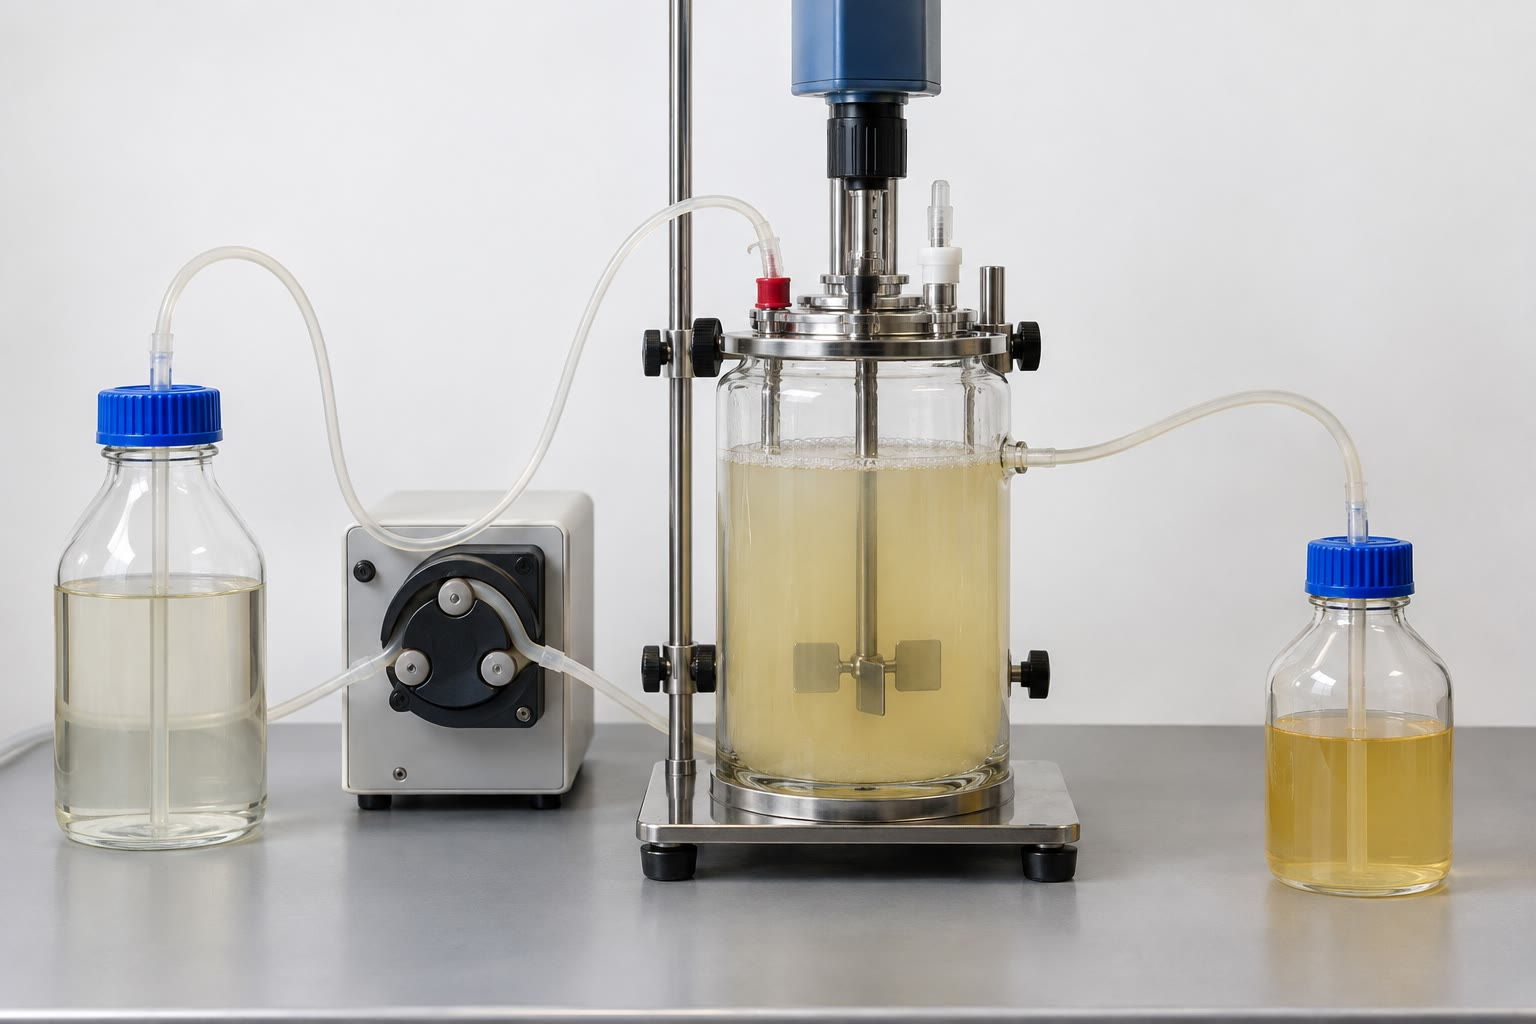
\includegraphics[width=0.6\linewidth]{images/book4/ai/b4-02-chemostat.jpg}

{\small Sebuah kemostat laboratorium: medium segar dipompa masuk dari
tandon di sebelah kiri, biakannya melimpah keluar ke kanan; pompanya
menetapkan laju pertumbuhannya.}
\end{omfigure}

\begin{example}[Membaca sebuah kemostat]\label{ex:b2:microbial-metabolism:chemostat}
Dengan $\mu_{\max} = \qty{1.0}{h^{-1}}$, $K_s = \qty{0.02}{g/L}$,
$S_{\text{masuk}} = \qty{2}{g/L}$ dan $Y = 0.5$, pada $D =
\qty{0.5}{h^{-1}}$: $S^* = 0.02\times 0.5/0.5 = \qty{0.02}{g/L}$ dan
$X^* = 0.5\times 1.98 = \qty{0.99}{g/L}$; biakannya menyisakan
\qty{1}{\%} gulanya tanpa terpakai. Laju pencuciannya adalah $1.0\times
2/2.02 = \qty{0.99}{h^{-1}}$. Sebuah pencerna atau sebuah usus bekerja
dengan asas yang sama: usus besar manusia, yang disuapi tiga kali
sehari dan dikosongkan sekali, menahan bakterinya pada \omterm{thm:b2:microbial-metabolism:chemostat}{laju
pengenceran} sekitar \qty{0.04}{h^{-1}}, dan setiap spesies yang tidak
sanggup berlipat dua dalam sehari akan tercuci keluar --- kecuali kalau
ia berpegang pada dindingnya.
\end{example}

\section{Biofilm}

\begin{definition}[Biofilm]\label{def:b2:microbial-metabolism:biofilm}
\index{biofilm}\index{matriks ekstrasel!bakteri}
Sebuah \emph{biofilm} adalah paguyuban mikroorganisme yang melekat pada
sebuah permukaan dan terbenam di dalam \emph{matriks} polisakarida,
protein, serta DNA ekstrasel yang dihasilkannya sendiri. Ia terbentuk
dalam beberapa tahap: \emph{pelekatan} sel tunggal yang masih dapat
balik (flagelum, pili), pelekatan tak terbalikkan dan pertumbuhan
\emph{mikrokoloni}, \emph{pematangan} menjadi lapisan terstruktur
bermenara dan berkanal air, serta \emph{penyebaran} sel yang berenang
pergi menyemai permukaan baru. Matriksnya menahan air dan hara,
melindungi selnya dari pengeringan, pemangsa, antibiotik, dan sel imun,
serta membangun landaian kimia yang menjadikan lapisan itu sebuah
bentang relung. Sebagian besar bakteri di Bumi hidup dengan cara ini:
pada batu di sungai, pada akar, pada gigi (plak gigi), pada kateter dan
implan, di dalam paru-paru penderita fibrosis kistik, pada lambung
kapal, dan di dalam pipa.
\end{definition}

\begin{omfigure}
\begin{tikzpicture}[every node/.style={font=\scriptsize}]
  \fill[gray!35] (0,0) rectangle (13.6,0.35);
  \node at (6.8,0.17) {permukaan};
  % stage 1 attachment
  \foreach \p in {(0.6,0.55),(1.4,0.55)} \draw[thick, omDef, fill=omDef!30] \p ellipse (0.22 and 0.1);
  \draw[thick, omDef, fill=omDef!30] (1.0,1.6) ellipse (0.22 and 0.1);
  \draw[->, omDef] (1.0,1.45) -- (1.0,0.75);
  \node[below, align=center] at (1.1,-0.05) {1. pelekatan};
  % stage 2 microcolony
  \begin{scope}[xshift=3.4cm]
    \fill[omExo!25] (0.15,0.35) .. controls (0.1,1.1) and (1.5,1.1) .. (1.45,0.35);
    \foreach \p in {(0.45,0.5),(0.8,0.5),(1.15,0.5),(0.6,0.75),(0.95,0.75),(0.8,0.95)} \draw[thick, omDef, fill=omDef!30] \p ellipse (0.18 and 0.09);
    \node[below, align=center] at (0.8,-0.05) {2. mikrokoloni,\\sekresi matriks};
  \end{scope}
  % stage 3 mature with channels
  \begin{scope}[xshift=6.8cm]
    \fill[omExo!25] (0.0,0.35) .. controls (0.2,1.9) and (0.9,2.2) .. (1.1,1.5) .. controls (1.2,0.9) and (1.4,0.6) .. (1.5,0.35);
    \fill[omExo!25] (1.7,0.35) .. controls (1.6,1.5) and (2.6,2.3) .. (2.9,1.2) .. controls (3.0,0.8) and (3.1,0.5) .. (3.2,0.35);
    \foreach \p in {(0.35,0.55),(0.7,0.55),(0.5,0.85),(0.8,1.15),(0.55,1.45),(2.0,0.6),(2.4,0.6),(2.2,0.9),(2.5,1.25),(2.3,1.6),(2.6,1.9),(2.1,1.3)} \draw[thick, omDef, fill=omDef!30] \p ellipse (0.16 and 0.08);
    \draw[<->, omThm, thick] (1.6,0.5) -- (1.6,1.6);
    \node[omThm, anchor=south] at (1.6,2.45) {kanal air};
    \node[below, align=center] at (1.6,-0.05) {3. lapisan matang: menara,\\kanal, landaian};
  \end{scope}
  % stage 4 dispersal
  \begin{scope}[xshift=11.2cm]
    \fill[omExo!25] (0.0,0.35) .. controls (0.1,1.5) and (1.0,1.6) .. (1.1,0.35);
    \foreach \p in {(0.3,0.55),(0.65,0.55),(0.5,0.85)} \draw[thick, omDef, fill=omDef!30] \p ellipse (0.16 and 0.08);
    \foreach \p/\a in {(1.4,1.5)/40,(1.9,1.1)/10,(1.6,2.0)/70} \draw[thick, omDef, fill=omDef!30, rotate around={\a:\p}] \p ellipse (0.16 and 0.08);
    \draw[->, omDef] (1.0,1.0) -- (1.35,1.35);
    \node[below, align=center] at (1.0,-0.05) {4. penyebaran};
  \end{scope}
\end{tikzpicture}

{\small Daur hidup sebuah \omterm{def:b2:microbial-metabolism:biofilm}{biofilm}: sel tunggal melekat, tumbuh menjadi
mikrokoloni yang menyekresikan matriks (kelabu), matang menjadi lapisan
terstruktur bermenara dan berkanal air, lalu melepaskan sel berenang
yang menjajah permukaan baru.}
\end{omfigure}

\begin{omfigure}
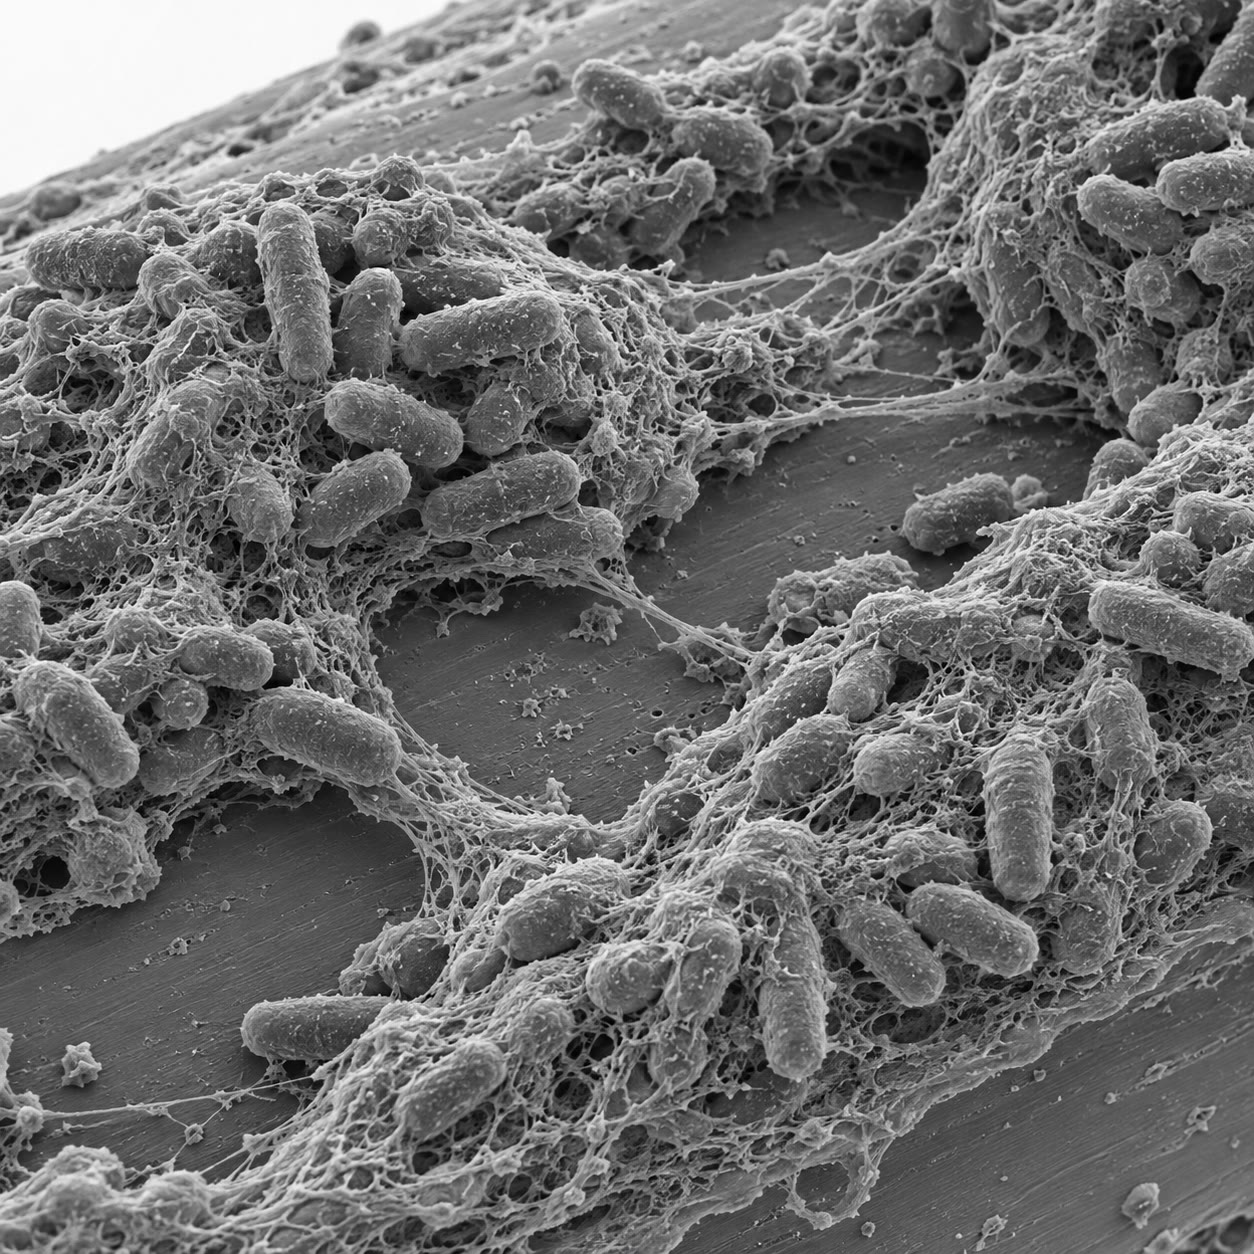
\includegraphics[width=0.46\linewidth]{images/book4/ai/b4-02-biofilm-sem.jpg}

{\small Sebuah \omterm{def:b2:microbial-metabolism:biofilm}{biofilm} pada sebuah kateter, dilihat dengan mikroskopi
elektron payaran: bakteri berbentuk batang terbenam di dalam matriks
berserat yang mereka sekresikan, dengan kanal terbuka di antara
gerombolannya.}
\end{omfigure}

\begin{theorem}[Landaian di dalam sebuah biofilm]\label{thm:b2:microbial-metabolism:gradient}
\index{kedalaman tembus oksigen}
Di dalam lapisan setebal $L$ yang selnya memakai oksigen pada laju
volumetrik tetap $q$, dengan kepekatannya ditahan pada $c_0$ di
permukaannya dan tanpa fluks menembus alasnya, tampang oksigen keadaan
tunaknya berbentuk parabola, dan jika lapisannya cukup tebal sehingga
oksigennya habis, hal itu terjadi pada \emph{kedalaman tembus}
\[
L_p = \sqrt{\frac{2 D_e\, c_0}{q}},
\]
dengan $D_e$ sebagai koefisien difusi efektif di dalam matriksnya.
Dengan $D_e = \qty{1.5e-9}{m^2/s}$, $c_0 = \qty{0.25}{mol/m^3}$ dan $q
= \qty{0.17}{mol/m^3/s}$ (lapisan padat berisi sel yang bernapas), $L_p
\approx \qty{66}{\micro m}$: di bawah sepersepuluh milimeter sebuah \omterm{def:b2:microbial-metabolism:biofilm}{biofilm}
kehabisan oksigen, dan penitrifikasi balik, pefermentasi, serta
pereduksi sulfat hidup di bawah atap kaum aerob.
\end{theorem}
\begin{proof}
Misalkan $x$ adalah kedalaman di bawah permukaannya. Pada keadaan tunak
fluks difusifnya $-D_e\,\mathrm{d}c/\mathrm{d}x$ berubah menurut
kedalaman hanya oleh pemakaiannya: $D_e\,\mathrm{d}^2c/\mathrm{d}x^2 = q$.
Mengintegralkan dua kali, $c = c_0 + a x + q x^2/2D_e$. Jika oksigennya
lenyap pada kedalaman $L_p$ dengan fluks nol di situ (tidak ada yang
datang dari bawah), $c(L_p) = 0$ dan $c'(L_p) = 0$: yang kedua memberi
$a = -qL_p/D_e$, dan yang pertama lalu memberi
$c_0 - qL_p^2/D_e + qL_p^2/2D_e = 0$, yakni $L_p^2 = 2D_e c_0/q$.
Tampangnya adalah
$c = (q/2D_e)(L_p - x)^2$.
\end{proof}

\begin{omfigure}
\begin{tikzpicture}
\begin{axis}[
  width=0.78\linewidth, height=5.6cm,
  axis x line=bottom, axis y line=left,
  xmin=0, xmax=120, ymin=0, ymax=0.28,
  xlabel={kedalaman di dalam lapisan (\unit{\micro m})}, ylabel={$\mathrm{O_2}$ (\unit{mol/m^3})},
  xlabel style={font=\small, at={(axis description cs:0.5,-0.14)}, anchor=north},
  ylabel style={font=\small},
  tick label style={font=\small}, xtick={0,20,40,60,80,100,120}, ytick={0,0.1,0.2},
  clip=false,
]
\addplot[very thick, omDef, domain=0:66, samples=60] {0.25*(1-x/66)^2};
\addplot[very thick, omDef, domain=66:120, samples=2] {0};
\fill[omThm!12] (axis cs:66,0) rectangle (axis cs:120,0.28);
\node[font=\scriptsize, anchor=north, align=center] at (axis cs:93,0.27) {zona tanpa oksigen:\\penitrifikasi balik, pefermentasi,\\pereduksi sulfat};
\draw[dashed, gray] (axis cs:66,0) -- (axis cs:66,0.28); \node[font=\scriptsize, anchor=south] at (axis cs:66,0.28) {$L_p$};
\node[font=\scriptsize, anchor=west] at (axis cs:24,0.18) {zona aerob};
\end{axis}
\end{tikzpicture}

{\small Oksigen di dalam sebuah \omterm{def:b2:microbial-metabolism:biofilm}{biofilm} yang bernapas: penurunan
parabolik dari nilai ruahnya di permukaan sampai nol pada kedalaman
tembusnya, \qty{66}{\micro m} bagi angka teoremanya. Semua yang lebih
dalam kehabisan oksigen.}
\end{omfigure}

\begin{proposition}[Penginderaan kuorum]\label{prop:b2:microbial-metabolism:quorum}
\index{penginderaan kuorum}\index{autoinduser}
Bakteri mencacah dirinya sendiri. Tiap selnya menyekresikan sebuah
molekul isyarat kecil, yaitu sebuah \emph{autoinduser} (asil-homoserina
lakton pada Gram negatif, peptida pendek pada Gram positif), pada laju
tetap yang rendah. Di dalam suspensi encer isyaratnya berdifusi pergi;
di dalam populasi padat atau sebuah \omterm{def:b2:microbial-metabolism:biofilm}{biofilm} ia menimbun, dan di atas
kepekatan ambang ia mengikat sebuah reseptor yang menyalakan seperangkat
gen --- termasuk gen autoinduser itu sendiri, dan dari situlah namanya.
Gen yang dikendalikan begitu adalah gen yang hanya berbayar kalau
banyak sel bertindak bersama: pendaran, sekresi enzim pencerna dan
racun, pembuatan matriks, serta keganasan patogen yang harus
menenggelamkan inangnya sekaligus alih-alih menyiagakannya satu sel
demi satu sel.
\end{proposition}
\begin{proof}[Bukti eksperimental]
Nealson, Platt, dan Hastings (1970) mendapati bahwa bakteri laut
\emph{Vibrio fischeri}, yang menerangi organ seekor cumi-cumi, gelap di
dalam biakan encer dan hanya berpendar di atas sekitar $10^{7}$ sel
tiap mililiter; medium bebas sel yang diambil dari biakan padat yang
berpendar membuat biakan encer berpendar seketika. Mediumnya memuat
isyaratnya; strukturnya, sebuah asil-homoserina lakton, ditetapkan pada
1981, dan mutan yang tak sanggup membuatnya tidak pernah berpendar
sepadat apa pun mereka jadinya.
\end{proof}

\begin{example}[Mengapa sebuah biofilm selamat dari antibiotik]\label{ex:b2:microbial-metabolism:tolerance}
Sel di dalam sebuah \omterm{def:b2:microbial-metabolism:biofilm}{biofilm} selamat dari kepekatan antibiotik seratus
sampai seribu kali kepekatan yang membunuh galur yang sama di dalam
suspensi, tanpa gen kekebalan apa pun. Matriksnya memperlambat difusi
obatnya dan mengikat sebagiannya; landaiannya membuat sel yang dalam
kelaparan, kehabisan oksigen, dan nyaris tidak tumbuh, sedangkan
kebanyakan antibiotik hanya membunuh sel yang tumbuh (penisilin
membutuhkan sintesis dinding, aminoglikosida membutuhkan pengangkutan
aktif); beberapa sel \emph{pembandel} bahkan dorman seluruhnya dan
menumbuhkan kembali lapisannya ketika pengobatannya berhenti. Maka
jangkitan menahun pada sebuah implan biasanya diobati dengan mencabut
implannya.
\end{example}

\section{Paguyuban mikroba}

\begin{example}[Tabung Winogradsky, dijelaskan]\label{ex:b2:microbial-metabolism:column}
Cahaya dan udara masuk dari atas; bahan organik dan sulfat dari
lumpurnya. Sianobakteri dan alga tumbuh di puncaknya lalu melepaskan
oksigen. Di bawahnya, heterotrof menghabiskan oksigennya pada bahan
organiknya, lalu nitratnya; lebih dalam lagi, pereduksi sulfat mengubah
sulfat menjadi sulfida, yang berdifusi ke atas dan menghitamkan
lumpurnya dengan besi sulfida. Di tempat sulfida yang naik bertemu
cahaya yang turun, bakteri belerang ungu mengoksidasinya secara
fotosintetik (pita ungunya), bakteri belerang hijau di bawahnya; di
tempat sulfida bertemu oksigen, dalam gelap, pengoksidasi belerang tak
berwarna seperti \emph{Beggiatoa} mencari nafkah secara \omterm{def:b2:microbial-metabolism:trophic}{kemolitotrofik}
(selubung putihnya); di tempat besi tereduksi bertemu oksigen,
pengoksidasi besi meninggalkan pita berkarat. Belerang berdaur antara
sulfida dan sulfat di dalam tabungnya; karbon berdaur antara
$\mathrm{CO_2}$ dan bahan organik; hanya cahaya yang masuk dan hanya
bahang yang keluar. Ia adalah ekosistem tertutup dengan neraca energi
terbuka, dan sebuah model berskala dasar samudra.
\end{example}

\begin{omfigure}
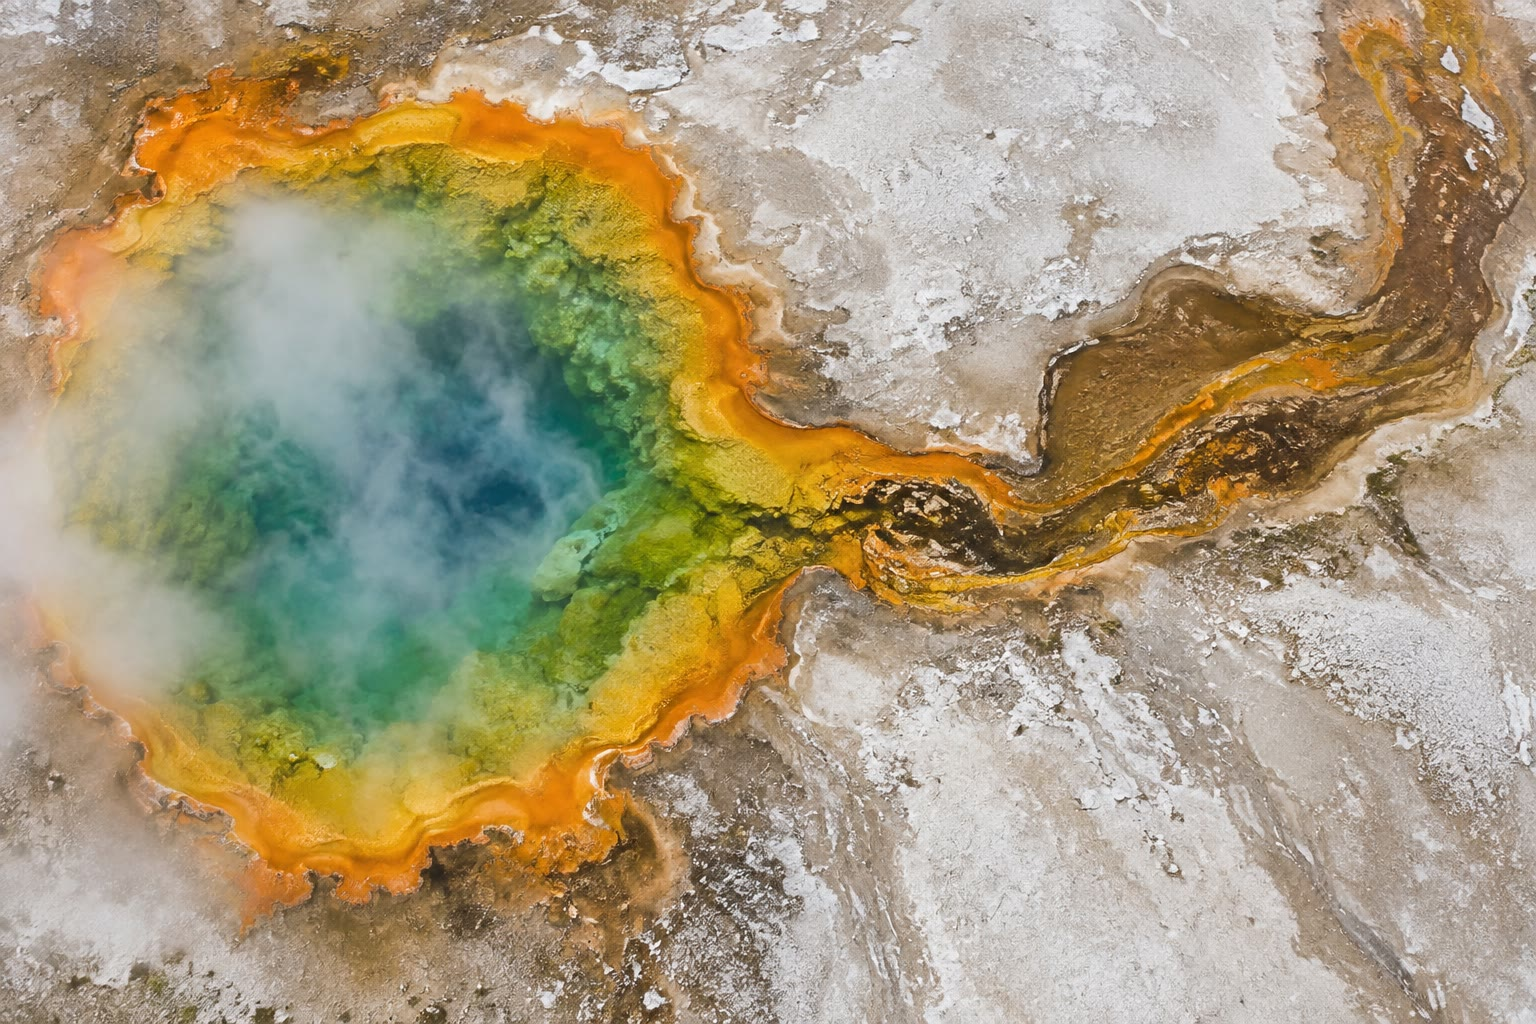
\includegraphics[width=0.62\linewidth]{images/book4/ai/b4-02-hot-spring-mats.jpg}

{\small Hamparan mikroba di sekitar sebuah mata air panas: tiap warnanya
adalah satu populasi yang hidup pada suhu dan kimia pitanya sendiri ---
sianobakteri dan bakteri hijau termofilik di aliran keluar yang lebih
sejuk, \omterm{def:b2:microbial-metabolism:trophic}{kemolitotrof} tak berwarna di air yang terpanas.}
\end{omfigure}

\begin{remark}[Hamparan mikroba dan Bumi purba]\label{rem:b2:microbial-metabolism:mats}
Di sekitar mata air panas dan di atas paparan pasang surut, hamparan
mikroba berlapis setebal beberapa milimeter memampatkan seluruh
tabungnya ke dalam ketebalan yang dapat dilintasi cahaya: sianobakteri
di atas, bakteri ungu di bawahnya, pereduksi sulfat di dasarnya, tiap
lapisnya memakan apa yang dihasilkan lapis di atasnya, dan hamparannya
merayap naik menembus endapan yang dijeratnya. Hamparan fosil ---
stromatolit --- adalah bukti kehidupan yang tertua, berumur \num{3.5}
miliar tahun. Selama dua miliar tahun, sebelum ada tumbuhan atau hewan,
biosfernya adalah hamparan ini dan plankton di atasnya, dan merekalah
yang memenuhi udara dengan oksigen
(\cref{ch:b2:biogeochemical-cycles}).
\end{remark}

\section{Latihan}

\begin{exercise}[$\star$]\label{exo:b2:microbial-metabolism:1}
Golongkanlah menurut sumber energi, sumber elektron, dan sumber karbon:
sebuah sianobakteri; \emph{Nitrosomonas}; \emph{E.~coli} pada glukosa;
sebuah bakteri ungu nirbelerang yang tumbuh dalam cahaya pada suksinat;
\emph{Thiobacillus} pada $\mathrm{H_2S}$ di dalam gelap.
\end{exercise}

\begin{exercise}[$\star$]\label{exo:b2:microbial-metabolism:2}
Daftarkanlah penerima elektron respirasi menurut urutan hasil energinya
yang menurun, dan katakan di bagian mana endapan masing-masing dipakai.
\end{exercise}

\begin{exercise}[$\star$]\label{exo:b2:microbial-metabolism:3}
Setarakanlah oksidasi glukosa menjadi $\mathrm{CO_2}$ oleh nitrat yang
tereduksi menjadi $\mathrm{N_2}$ (dalam larutan asam, dengan air sebagai
hasil yang lain). Berapa ion nitrat tiap glukosanya?
\end{exercise}

\begin{exercise}[$\star$]\label{exo:b2:microbial-metabolism:4}
Definisikan sebuah \omterm{def:b2:microbial-metabolism:biofilm}{biofilm} lalu sebutkan keempat tahapnya. Berikan tiga
tempat \omterm{def:b2:microbial-metabolism:biofilm}{biofilm} berarti bagi kesehatan manusia atau industri.
\end{exercise}

\begin{exercise}[$\star\star$]\label{exo:b2:microbial-metabolism:5}
Hitunglah $\Delta G^{\circ\prime}$ bagi $4\mathrm{H_2} + \mathrm{CO_2}
\to \mathrm{CH_4} + 2\mathrm{H_2O}$ dari potensial
$\mathrm{2H^+/H_2}$ (\qty{-0.42}{V}) dan $\mathrm{CO_2/CH_4}$
(\qty{-0.24}{V}). Paling banyak berapa ATP (pada \qty{50}{kJ/mol}) yang
dapat dibuat seorang metanogen tiap $\mathrm{H_2}$? Ulaslah laju
pertumbuhannya.
\end{exercise}

\begin{exercise}[$\star\star$]\label{exo:b2:microbial-metabolism:6}
Sebuah bakteri memiliki $\mu_{\max} = \qty{1.2}{h^{-1}}$ dan $K_s =
\qty{5}{mg/L}$ glukosa. Hitunglah $\mu$ dan \omterm{def:b2:unicellular-diversity:division}{waktu generasinya} pada
1, 5, dan \qty{50}{mg/L}. Pada kepekatan berapa ia tumbuh pada
\qty{90}{\%} maksimumnya?
\end{exercise}

\begin{exercise}[$\star\star$]\label{exo:b2:microbial-metabolism:7}
Sebuah kemostat dengan $\mu_{\max} = \qty{0.8}{h^{-1}}$, $K_s =
\qty{0.05}{g/L}$, $S_{\text{masuk}} = \qty{5}{g/L}$, $Y = 0.4$ berjalan pada
$D = \qty{0.4}{h^{-1}}$. Hitunglah $S^*$, $X^*$, keluaran biomassa
tiap liter tiap jam, dan laju pencuciannya.
\end{exercise}

\begin{exercise}[$\star\star$]\label{exo:b2:microbial-metabolism:8}
Mengoksidasi satu $\mathrm{NH_4^+}$ menjadi nitrit menghasilkan
\qty{275}{kJ}; seorang penitrifikasi menangkap seperempatnya sebagai
ATP (\qty{50}{kJ/mol}), dan memfiksasi satu $\mathrm{CO_2}$ menjadi
biomassa memakan setara 12 ATP. Berapa ion amonium yang harus
dioksidasinya tiap karbon yang difiksasi? Mengapa hasil seorang
penitrifikasi begitu rendah dibandingkan dengan hasil seorang heterotrof?
\end{exercise}

\begin{exercise}[$\star\star$]\label{exo:b2:microbial-metabolism:9}
Hitunglah \omterm{thm:b2:microbial-metabolism:gradient}{kedalaman tembus oksigen} di dalam sebuah \omterm{def:b2:microbial-metabolism:biofilm}{biofilm} dengan $D_e =
\qty{1.2e-9}{m^2/s}$, $c_0 = \qty{0.20}{mol/m^3}$ dan $q =
\qty{0.5}{mol/m^3/s}$. Apa yang terjadi pada $L_p$ jika oksigen ruahnya
dilipatduakan? Jika selnya bernapas empat kali lebih cepat?
\end{exercise}

\begin{exercise}[$\star\star\star$]\label{exo:b2:microbial-metabolism:10}
Ramalkanlah pita-pita sebuah tabung Winogradsky dari atas ke bawah,
sambil menamai metabolisme masing-masing, lalu jelaskan (a) mengapa pita
ungunya terbentuk di tempat ia terbentuk, (b) mengapa lumpurnya menjadi
hitam, (c) dalam arti apa tabungnya sebuah sistem tertutup dan dalam
arti apa ia sebuah sistem terbuka.
\end{exercise}

\begin{exercise}[$\star\star\star$]\label{exo:b2:microbial-metabolism:11}
Tiap sel sebuah populasi berkerapatan $n$ (sel tiap liter) menyekresikan
sebuah autoinduser pada $p = 5$ molekul tiap sekon; molekulnya
terurai pada laju $k = \qty{5e-4}{s^{-1}}$. Tuliskanlah kepekatan
keadaan tunaknya $A^*$ sebagai fungsi $n$. Reseptornya menyala pada
$A_c = \qty{10}{nmol/L}$: hitunglah kerapatan ambangnya dalam sel tiap
mililiter. Bandingkan dengan biakan padat ($10^{9}$ tiap mililiter) dan
dengan air laut ($10^{5}$ tiap mililiter), lalu jelaskan mengapa sebuah
\omterm{def:b2:microbial-metabolism:biofilm}{biofilm} mencapai kuorum di dalam volume yang tidak akan pernah dicapai
sebuah suspensi.
\end{exercise}

\begin{exercise}[$\star\star\star$]\label{exo:b2:microbial-metabolism:12}
``\omterm{def:b2:unicellular-diversity:prokaryote}{Prokariot} menjalankan kimia planet ini.'' Bahaslah dengan tiga proses
dari bab ini yang tidak dapat dikerjakan eukariot mana pun, sambil
mengatakan untuk masing-masing apa yang akan terjadi pada biosfernya
jika proses itu berhenti.
\end{exercise}

\section{Soal: Sebuah Instalasi Pengolahan Air Limbah}

\begin{problem}[{Soal akhir pekan --- limbah sebuah kota dianalisis
sebagai seperangkat reaktor mikroba, dari energetika bakterinya sampai
metana yang menenagainya, berakhir pada neraca energi instalasinya}]
\label{pb:b2:microbial-metabolism:1}
Sebuah instalasi mengolah $Q = \qty{10000}{m^3}$ air limbah sehari yang
mengusung \qty{300}{g/m^3} bahan organik, diukur sebagai oksigen yang
dibutuhkan untuk membakarnya (\emph{kebutuhan oksigen kimiawi}, COD),
dan \qty{40}{g/m^3} nitrogen amonium. Ia memiliki sebuah tangki lumpur
aktif beraerasi, sebuah tangki tanpa oksigen untuk \omterm{def:b2:microbial-metabolism:anaerobic}{denitrifikasi}, dan
sebuah pencerna anaerob untuk lumpurnya. Data: heterotrof aerob
mengubah bahan organik dengan hasil $Y = 0.4$ (kilogram COD biomassa
tiap kilogram COD substrat, sehingga sisanya teroksidasi);
nitrifikasi membutuhkan \qty{4.57}{kg} $\mathrm{O_2}$ tiap kilogram
nitrogen; \omterm{def:b2:microbial-metabolism:anaerobic}{denitrifikasi} membutuhkan \qty{2.86}{kg} COD substrat tiap
kilogram nitrogen nitrat; aerasi mengantarkan \qty{2}{kg}
$\mathrm{O_2}$ tiap kilowatt-jam; COD lumpurnya diubah menjadi
metana di dalam pencernanya sebesar \qty{60}{\%}, tiap kilogram COD
yang terubah memberikan \qty{0.35}{m^3} metana berkandungan energi
\qty{36}{MJ/m^3}, yang dibakar dalam generator berefisiensi listrik
\qty{35}{\%}. Penitrifikasi: $\mu_{\max} = \qty{0.5}{d^{-1}}$, $K_s =
\qty{1}{g/m^3}$ nitrogen amonium.

\medskip
\noindent\textbf{Bagian I --- Energetikanya.}
\begin{enumerate}
  \item Dengan memakai \omterm{thm:b2:microbial-metabolism:redox}{menara elektron}, hitunglah $\Delta G^{\circ\prime}$
        bagi oksidasi satu mol glukosa (24 elektron pada
        \qty{-0.43}{V}) oleh oksigen (\qty{+0.82}{V}).
  \item Hitunglah nilainya bagi nitrat yang tereduksi menjadi $\mathrm{N_2}$
        (\qty{+0.74}{V}) dan bagi sulfat yang tereduksi menjadi sulfida
        (\qty{-0.22}{V}).
  \item Mengapa \omterm{def:b2:microbial-metabolism:anaerobic}{denitrifikasi} baru mulai di dalam tangki tanpa oksigen, dan
        mengapa \omterm{def:b2:microbial-metabolism:anaerobic}{reduksi sulfat} (dengan baunya) adalah tanda instalasi
        yang buruk pengelolaannya?
  \item Jika sel menangkap \qty{40}{\%} energi bebasnya sebagai ATP
        (\qty{50}{kJ/mol}), berapa ATP tiap glukosa yang diberikan
        masing-masing dari ketiga metabolisme itu?
  \item Berapa kali lebih banyak glukosa yang harus diolah seorang
        pereduksi sulfat daripada seorang aerob demi pertumbuhan yang sama?
  \item Pefermentasi di dalam pencernanya memperoleh 2 ATP tiap glukosa.
        Jelaskan mengapa pencernanya tetap saja menghasilkan biomassa
        yang hampir nol dan kebanyakan gas.
\end{enumerate}

\medskip
\noindent\textbf{Bagian II --- Tangki beraerasi.}
\begin{enumerate}[resume]
  \item Hitunglah beban bahan organik hariannya, dalam kilogram COD.
  \item Hitunglah biomassa yang dihasilkan tiap hari (sebagai COD) dan
        oksigen yang dibutuhkan untuk mengoksidasi sisanya.
  \item Hitunglah energi aerasi bagi bahan organiknya, dalam
        kilowatt-jam tiap hari.
  \item Hitunglah beban nitrogen hariannya dan oksigen yang dibutuhkan
        untuk menitrifikasinya.
  \item Lumpurnya ditahan di dalam tangkinya selama purata waktu $\theta$
        (kebalikan \omterm{thm:b2:microbial-metabolism:chemostat}{laju pengencerannya}). Di bawah $\theta$ berapa
        penitrifikasinya tercuci keluar pada kepekatan amonium berapa pun?
  \item Dengan $\theta = \qty{10}{d}$, hitunglah kepekatan amonium sisa
        di dalam efluennya.
  \item Musim dingin menurunkan $\mu_{\max}$ menjadi \qty{0.25}{d^{-1}}.
        Hitunglah kembali amonium sisanya lalu katakan apa yang harus
        dikerjakan operatornya.
\end{enumerate}

\medskip
\noindent\textbf{Bagian III --- \omterm{def:b2:microbial-metabolism:anaerobic}{Denitrifikasi} dan pencernanya.}
Nitrat yang dibuat di dalam tangki beraerasi didaurkan kembali ke tangki
tanpa oksigen, tempat heterotrof mereduksinya dengan bahan organik yang masuk.
\begin{enumerate}[resume]
  \item Hitunglah bahan organik (kilogram COD tiap hari) yang dipakai
        untuk mendenitrifikasi seluruh nitrogennya.
  \item Hitunglah massa nitrogen yang dilepaskan ke udara sebagai
        $\mathrm{N_2}$ tiap hari, dan massa yang pergi bersama efluennya
        sebagai amonium (pertanyaan 12), sebagai bagian dari bebannya.
  \item Bahan organik itu tidak lagi membutuhkan aerasi. Hitunglah
        oksigen yang dihemat, dan seluruh kebutuhan oksigen instalasinya
        (sisa bahan organik ditambah nitrifikasinya).
  \item Lumpur yang dihasilkan (pertanyaan 8, tetap sebagai COD) masuk ke
        pencernanya. Hitunglah metana yang dihasilkan tiap hari.
  \item Hitunglah energi metana itu dan listrik yang dihasilkannya.
  \item Hitunglah listrik aerasi bagi seluruh kebutuhan oksigen
        pertanyaan 16, lalu bandingkan.
\end{enumerate}

\medskip
\noindent\textbf{Bagian IV --- Reaktor \omterm{def:b2:microbial-metabolism:biofilm}{biofilm}.}
Sebuah saringan tetes menumbuhkan \omterm{def:b2:microbial-metabolism:biofilm}{biofilm} pada batu; air ruahnya memuat
\qty{0.2}{mol/m^3} oksigen, $D_e = \qty{1.5e-9}{m^2/s}$, dan
lapisannya bernapas pada $q = \qty{0.3}{mol/m^3/s}$.
\begin{enumerate}[resume]
  \item Turunkanlah tampang oksigen $c(x)$ di dalam lapisan yang cukup
        tebal untuk kehabisan oksigen.
  \item Hitunglah kedalaman tembusnya.
  \item Lapisannya setebal \qty{300}{\micro m}. Berapa bagiannya yang
        aerob, dan apa yang dikerjakan sel di bawahnya dengan nitrat
        yang berdifusi turun dari lapisan aerobnya?
  \item Jelaskan mengapa satu \omterm{def:b2:microbial-metabolism:biofilm}{biofilm} dapat menitrifikasi dan
        mendenitrifikasi sekaligus, yang tidak dapat dikerjakan tangki
        beraerasinya.
  \item Klorin ditambahkan untuk membasmi hama di dalam efluennya.
        Berikan dua alasan mengapa \omterm{def:b2:microbial-metabolism:biofilm}{biofilmnya} selamat dari takaran yang
        membunuh bakteri yang sama di dalam suspensi.
  \item Nyatakan hasilnya: kebutuhan oksigen harian instalasinya,
        keluaran metananya, dan bagian listrik aerasinya yang dipasok
        metananya.
\end{enumerate}
\end{problem}
